% Created by tikzDevice version 0.12.3.1 on 2021-12-15 13:57:49
% !TEX encoding = UTF-8 Unicode
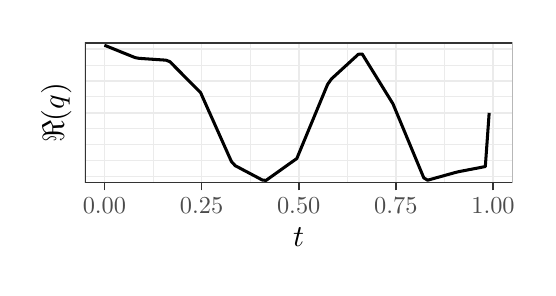
\begin{tikzpicture}[x=1pt,y=1pt]
\definecolor{fillColor}{RGB}{255,255,255}
\path[use as bounding box,fill=fillColor,fill opacity=0.00] (0,0) rectangle (180.67, 86.72);
\begin{scope}
\path[clip] (  0.00,  0.00) rectangle (180.67, 86.72);
\definecolor{drawColor}{RGB}{255,255,255}
\definecolor{fillColor}{RGB}{255,255,255}

\path[draw=drawColor,line width= 0.6pt,line join=round,line cap=round,fill=fillColor] (  0.00,  0.00) rectangle (180.67, 86.72);
\end{scope}
\begin{scope}
\path[clip] ( 20.71, 30.69) rectangle (175.17, 81.22);
\definecolor{fillColor}{RGB}{255,255,255}

\path[fill=fillColor] ( 20.71, 30.69) rectangle (175.17, 81.22);
\definecolor{drawColor}{gray}{0.92}

\path[draw=drawColor,line width= 0.3pt,line join=round] ( 20.71, 38.73) --
	(175.17, 38.73);

\path[draw=drawColor,line width= 0.3pt,line join=round] ( 20.71, 50.21) --
	(175.17, 50.21);

\path[draw=drawColor,line width= 0.3pt,line join=round] ( 20.71, 61.70) --
	(175.17, 61.70);

\path[draw=drawColor,line width= 0.3pt,line join=round] ( 20.71, 73.18) --
	(175.17, 73.18);

\path[draw=drawColor,line width= 0.3pt,line join=round] ( 45.29, 30.69) --
	( 45.29, 81.22);

\path[draw=drawColor,line width= 0.3pt,line join=round] ( 80.39, 30.69) --
	( 80.39, 81.22);

\path[draw=drawColor,line width= 0.3pt,line join=round] (115.50, 30.69) --
	(115.50, 81.22);

\path[draw=drawColor,line width= 0.3pt,line join=round] (150.60, 30.69) --
	(150.60, 81.22);

\path[draw=drawColor,line width= 0.6pt,line join=round] ( 20.71, 32.98) --
	(175.17, 32.98);

\path[draw=drawColor,line width= 0.6pt,line join=round] ( 20.71, 44.47) --
	(175.17, 44.47);

\path[draw=drawColor,line width= 0.6pt,line join=round] ( 20.71, 55.95) --
	(175.17, 55.95);

\path[draw=drawColor,line width= 0.6pt,line join=round] ( 20.71, 67.44) --
	(175.17, 67.44);

\path[draw=drawColor,line width= 0.6pt,line join=round] ( 20.71, 78.93) --
	(175.17, 78.93);

\path[draw=drawColor,line width= 0.6pt,line join=round] ( 27.74, 30.69) --
	( 27.74, 81.22);

\path[draw=drawColor,line width= 0.6pt,line join=round] ( 62.84, 30.69) --
	( 62.84, 81.22);

\path[draw=drawColor,line width= 0.6pt,line join=round] ( 97.94, 30.69) --
	( 97.94, 81.22);

\path[draw=drawColor,line width= 0.6pt,line join=round] (133.05, 30.69) --
	(133.05, 81.22);

\path[draw=drawColor,line width= 0.6pt,line join=round] (168.15, 30.69) --
	(168.15, 81.22);
\definecolor{drawColor}{RGB}{0,0,0}

\path[draw=drawColor,line width= 1.1pt,line join=round] ( 27.74, 80.38) --
	( 29.13, 79.82) --
	( 30.52, 79.26) --
	( 31.91, 78.70) --
	( 33.30, 78.13) --
	( 34.69, 77.57) --
	( 36.08, 77.01) --
	( 37.47, 76.45) --
	( 38.86, 75.89) --
	( 40.25, 75.64) --
	( 41.64, 75.54) --
	( 43.03, 75.45) --
	( 44.42, 75.35) --
	( 45.81, 75.26) --
	( 47.20, 75.16) --
	( 48.59, 75.07) --
	( 49.98, 74.97) --
	( 51.37, 74.44) --
	( 52.76, 73.04) --
	( 54.15, 71.64) --
	( 55.54, 70.24) --
	( 56.93, 68.83) --
	( 58.32, 67.43) --
	( 59.71, 66.03) --
	( 61.10, 64.63) --
	( 62.49, 63.23) --
	( 63.88, 60.12) --
	( 65.27, 57.01) --
	( 66.66, 53.91) --
	( 68.05, 50.80) --
	( 69.44, 47.69) --
	( 70.83, 44.59) --
	( 72.22, 41.48) --
	( 73.61, 38.37) --
	( 75.00, 36.85) --
	( 76.40, 36.11) --
	( 77.79, 35.37) --
	( 79.18, 34.64) --
	( 80.57, 33.90) --
	( 81.96, 33.17) --
	( 83.35, 32.43) --
	( 84.74, 31.69) --
	( 86.13, 31.53) --
	( 87.52, 32.52) --
	( 88.91, 33.51) --
	( 90.30, 34.50) --
	( 91.69, 35.49) --
	( 93.08, 36.48) --
	( 94.47, 37.47) --
	( 95.86, 38.45) --
	( 97.25, 39.44) --
	( 98.64, 42.79) --
	(100.03, 46.14) --
	(101.42, 49.49) --
	(102.81, 52.83) --
	(104.20, 56.18) --
	(105.59, 59.53) --
	(106.98, 62.88) --
	(108.37, 66.22) --
	(109.76, 68.19) --
	(111.15, 69.46) --
	(112.54, 70.74) --
	(113.93, 72.01) --
	(115.32, 73.28) --
	(116.71, 74.56) --
	(118.10, 75.83) --
	(119.49, 77.10) --
	(120.88, 77.20) --
	(122.27, 74.95) --
	(123.66, 72.69) --
	(125.06, 70.44) --
	(126.45, 68.18) --
	(127.84, 65.93) --
	(129.23, 63.67) --
	(130.62, 61.42) --
	(132.01, 59.16) --
	(133.40, 55.83) --
	(134.79, 52.49) --
	(136.18, 49.15) --
	(137.57, 45.81) --
	(138.96, 42.47) --
	(140.35, 39.13) --
	(141.74, 35.79) --
	(143.13, 32.46) --
	(144.52, 31.60) --
	(145.91, 31.99) --
	(147.30, 32.38) --
	(148.69, 32.76) --
	(150.08, 33.15) --
	(151.47, 33.54) --
	(152.86, 33.92) --
	(154.25, 34.31) --
	(155.64, 34.66) --
	(157.03, 34.93) --
	(158.42, 35.20) --
	(159.81, 35.47) --
	(161.20, 35.73) --
	(162.59, 36.00) --
	(163.98, 36.27) --
	(165.37, 36.54) --
	(166.76, 55.95);
\definecolor{drawColor}{gray}{0.20}

\path[draw=drawColor,line width= 0.6pt,line join=round,line cap=round] ( 20.71, 30.69) rectangle (175.17, 81.22);
\end{scope}
\begin{scope}
\path[clip] (  0.00,  0.00) rectangle (180.67, 86.72);
\definecolor{drawColor}{gray}{0.20}

\path[draw=drawColor,line width= 0.6pt,line join=round] ( 27.74, 27.94) --
	( 27.74, 30.69);

\path[draw=drawColor,line width= 0.6pt,line join=round] ( 62.84, 27.94) --
	( 62.84, 30.69);

\path[draw=drawColor,line width= 0.6pt,line join=round] ( 97.94, 27.94) --
	( 97.94, 30.69);

\path[draw=drawColor,line width= 0.6pt,line join=round] (133.05, 27.94) --
	(133.05, 30.69);

\path[draw=drawColor,line width= 0.6pt,line join=round] (168.15, 27.94) --
	(168.15, 30.69);
\end{scope}
\begin{scope}
\path[clip] (  0.00,  0.00) rectangle (180.67, 86.72);
\definecolor{drawColor}{gray}{0.30}

\node[text=drawColor,anchor=base,inner sep=0pt, outer sep=0pt, scale=  0.88] at ( 27.74, 19.68) {0.00};

\node[text=drawColor,anchor=base,inner sep=0pt, outer sep=0pt, scale=  0.88] at ( 62.84, 19.68) {0.25};

\node[text=drawColor,anchor=base,inner sep=0pt, outer sep=0pt, scale=  0.88] at ( 97.94, 19.68) {0.50};

\node[text=drawColor,anchor=base,inner sep=0pt, outer sep=0pt, scale=  0.88] at (133.05, 19.68) {0.75};

\node[text=drawColor,anchor=base,inner sep=0pt, outer sep=0pt, scale=  0.88] at (168.15, 19.68) {1.00};
\end{scope}
\begin{scope}
\path[clip] (  0.00,  0.00) rectangle (180.67, 86.72);
\definecolor{drawColor}{RGB}{0,0,0}

\node[text=drawColor,anchor=base,inner sep=0pt, outer sep=0pt, scale=  1.10] at ( 97.94,  7.64) {$t$};
\end{scope}
\begin{scope}
\path[clip] (  0.00,  0.00) rectangle (180.67, 86.72);
\definecolor{drawColor}{RGB}{0,0,0}

\node[text=drawColor,rotate= 90.00,anchor=base,inner sep=0pt, outer sep=0pt, scale=  1.10] at ( 13.08, 55.95) {$\Re(q)$};
\end{scope}
\end{tikzpicture}
